\documentclass[twoside]{book}

% Packages required by doxygen
\usepackage{fixltx2e}
\usepackage{calc}
\usepackage{doxygen}
\usepackage[export]{adjustbox} % also loads graphicx
\usepackage{graphicx}
\usepackage[utf8]{inputenc}
\usepackage{makeidx}
\usepackage{multicol}
\usepackage{multirow}
\PassOptionsToPackage{warn}{textcomp}
\usepackage{textcomp}
\usepackage[nointegrals]{wasysym}
\usepackage[table]{xcolor}

% Font selection
\usepackage[T1]{fontenc}
\usepackage[scaled=.90]{helvet}
\usepackage{courier}
\usepackage{amssymb}
\usepackage{sectsty}
\renewcommand{\familydefault}{\sfdefault}
\allsectionsfont{%
  \fontseries{bc}\selectfont%
  \color{darkgray}%
}
\renewcommand{\DoxyLabelFont}{%
  \fontseries{bc}\selectfont%
  \color{darkgray}%
}
\newcommand{\+}{\discretionary{\mbox{\scriptsize$\hookleftarrow$}}{}{}}

% Page & text layout
\usepackage{geometry}
\geometry{%
  a4paper,%
  top=2.5cm,%
  bottom=2.5cm,%
  left=2.5cm,%
  right=2.5cm%
}
\tolerance=750
\hfuzz=15pt
\hbadness=750
\setlength{\emergencystretch}{15pt}
\setlength{\parindent}{0cm}
\setlength{\parskip}{3ex plus 2ex minus 2ex}
\makeatletter
\renewcommand{\paragraph}{%
  \@startsection{paragraph}{4}{0ex}{-1.0ex}{1.0ex}{%
    \normalfont\normalsize\bfseries\SS@parafont%
  }%
}
\renewcommand{\subparagraph}{%
  \@startsection{subparagraph}{5}{0ex}{-1.0ex}{1.0ex}{%
    \normalfont\normalsize\bfseries\SS@subparafont%
  }%
}
\makeatother

% Headers & footers
\usepackage{fancyhdr}
\pagestyle{fancyplain}
\fancyhead[LE]{\fancyplain{}{\bfseries\thepage}}
\fancyhead[CE]{\fancyplain{}{}}
\fancyhead[RE]{\fancyplain{}{\bfseries\leftmark}}
\fancyhead[LO]{\fancyplain{}{\bfseries\rightmark}}
\fancyhead[CO]{\fancyplain{}{}}
\fancyhead[RO]{\fancyplain{}{\bfseries\thepage}}
\fancyfoot[LE]{\fancyplain{}{}}
\fancyfoot[CE]{\fancyplain{}{}}
\fancyfoot[RE]{\fancyplain{}{\bfseries\scriptsize Generated by Doxygen }}
\fancyfoot[LO]{\fancyplain{}{\bfseries\scriptsize Generated by Doxygen }}
\fancyfoot[CO]{\fancyplain{}{}}
\fancyfoot[RO]{\fancyplain{}{}}
\renewcommand{\footrulewidth}{0.4pt}
\renewcommand{\chaptermark}[1]{%
  \markboth{#1}{}%
}
\renewcommand{\sectionmark}[1]{%
  \markright{\thesection\ #1}%
}

% Indices & bibliography
\usepackage{natbib}
\usepackage[titles]{tocloft}
\setcounter{tocdepth}{3}
\setcounter{secnumdepth}{5}
\makeindex

% Hyperlinks (required, but should be loaded last)
\usepackage{ifpdf}
\ifpdf
  \usepackage[pdftex,pagebackref=true]{hyperref}
\else
  \usepackage[ps2pdf,pagebackref=true]{hyperref}
\fi
\hypersetup{%
  colorlinks=true,%
  linkcolor=blue,%
  citecolor=blue,%
  unicode%
}

% Custom commands
\newcommand{\clearemptydoublepage}{%
  \newpage{\pagestyle{empty}\cleardoublepage}%
}

\usepackage{caption}
\captionsetup{labelsep=space,justification=centering,font={bf},singlelinecheck=off,skip=4pt,position=top}

%===== C O N T E N T S =====

\begin{document}

% Titlepage & ToC
\hypersetup{pageanchor=false,
             bookmarksnumbered=true,
             pdfencoding=unicode
            }
\pagenumbering{alph}
\begin{titlepage}
\vspace*{7cm}
\begin{center}%
{\Large Day 448 -\/ E\+E\+CS 448 Project 3 }\\
\vspace*{1cm}
{\large Generated by Doxygen 1.8.14}\\
\end{center}
\end{titlepage}
\clearemptydoublepage
\pagenumbering{roman}
\tableofcontents
\clearemptydoublepage
\pagenumbering{arabic}
\hypersetup{pageanchor=true}

%--- Begin generated contents ---
\chapter{Hierarchical Index}
\section{Class Hierarchy}
This inheritance list is sorted roughly, but not completely, alphabetically\+:\begin{DoxyCompactList}
\item \contentsline{section}{Map\+Bounds}{\pageref{class_map_bounds}}{}
\item Mono\+Behaviour\begin{DoxyCompactList}
\item \contentsline{section}{asteroid\+Mover}{\pageref{classasteroid_mover}}{}
\item \contentsline{section}{asteroid\+Rotator}{\pageref{classasteroid_rotator}}{}
\item \contentsline{section}{B\+G\+Scroller}{\pageref{class_b_g_scroller}}{}
\item \contentsline{section}{destroy\+Asteroid}{\pageref{classdestroy_asteroid}}{}
\item \contentsline{section}{destroyby\+Time}{\pageref{classdestroyby_time}}{}
\item \contentsline{section}{Game\+Controller}{\pageref{class_game_controller}}{}
\item \contentsline{section}{laser\+Movement}{\pageref{classlaser_movement}}{}
\item \contentsline{section}{out\+Of\+Bounds}{\pageref{classout_of_bounds}}{}
\item \contentsline{section}{Player\+Controller}{\pageref{class_player_controller}}{}
\end{DoxyCompactList}
\end{DoxyCompactList}

\chapter{Class Index}
\section{Class List}
Here are the classes, structs, unions and interfaces with brief descriptions\+:\begin{DoxyCompactList}
\item\contentsline{section}{\mbox{\hyperlink{classasteroid_mover}{asteroid\+Mover}} }{\pageref{classasteroid_mover}}{}
\item\contentsline{section}{\mbox{\hyperlink{classasteroid_rotator}{asteroid\+Rotator}} }{\pageref{classasteroid_rotator}}{}
\item\contentsline{section}{\mbox{\hyperlink{class_b_g_scroller}{B\+G\+Scroller}} }{\pageref{class_b_g_scroller}}{}
\item\contentsline{section}{\mbox{\hyperlink{classdestroy_asteroid}{destroy\+Asteroid}} }{\pageref{classdestroy_asteroid}}{}
\item\contentsline{section}{\mbox{\hyperlink{classdestroyby_time}{destroyby\+Time}} }{\pageref{classdestroyby_time}}{}
\item\contentsline{section}{\mbox{\hyperlink{class_game_controller}{Game\+Controller}} }{\pageref{class_game_controller}}{}
\item\contentsline{section}{\mbox{\hyperlink{classlaser_movement}{laser\+Movement}} }{\pageref{classlaser_movement}}{}
\item\contentsline{section}{\mbox{\hyperlink{class_map_bounds}{Map\+Bounds}} }{\pageref{class_map_bounds}}{}
\item\contentsline{section}{\mbox{\hyperlink{classout_of_bounds}{out\+Of\+Bounds}} }{\pageref{classout_of_bounds}}{}
\item\contentsline{section}{\mbox{\hyperlink{class_player_controller}{Player\+Controller}} }{\pageref{class_player_controller}}{}
\end{DoxyCompactList}

\chapter{File Index}
\section{File List}
Here is a list of all files with brief descriptions\+:\begin{DoxyCompactList}
\item\contentsline{section}{\mbox{\hyperlink{asteroid_mover_8cs}{asteroid\+Mover.\+cs}} }{\pageref{asteroid_mover_8cs}}{}
\item\contentsline{section}{\mbox{\hyperlink{asteroid_rotator_8cs}{asteroid\+Rotator.\+cs}} }{\pageref{asteroid_rotator_8cs}}{}
\item\contentsline{section}{\mbox{\hyperlink{_b_g_scroller_8cs}{B\+G\+Scroller.\+cs}} }{\pageref{_b_g_scroller_8cs}}{}
\item\contentsline{section}{\mbox{\hyperlink{destroy_asteroid_8cs}{destroy\+Asteroid.\+cs}} }{\pageref{destroy_asteroid_8cs}}{}
\item\contentsline{section}{\mbox{\hyperlink{destroyby_time_8cs}{destroyby\+Time.\+cs}} }{\pageref{destroyby_time_8cs}}{}
\item\contentsline{section}{\mbox{\hyperlink{_game_controller_8cs}{Game\+Controller.\+cs}} }{\pageref{_game_controller_8cs}}{}
\item\contentsline{section}{\mbox{\hyperlink{laser_movement_8cs}{laser\+Movement.\+cs}} }{\pageref{laser_movement_8cs}}{}
\item\contentsline{section}{\mbox{\hyperlink{out_of_bounds_8cs}{out\+Of\+Bounds.\+cs}} }{\pageref{out_of_bounds_8cs}}{}
\item\contentsline{section}{\mbox{\hyperlink{_player_controller_8cs}{Player\+Controller.\+cs}} }{\pageref{_player_controller_8cs}}{}
\end{DoxyCompactList}

\chapter{Class Documentation}
\hypertarget{classasteroid_mover}{}\section{asteroid\+Mover Class Reference}
\label{classasteroid_mover}\index{asteroid\+Mover@{asteroid\+Mover}}
Inheritance diagram for asteroid\+Mover\+:\begin{figure}[H]
\begin{center}
\leavevmode
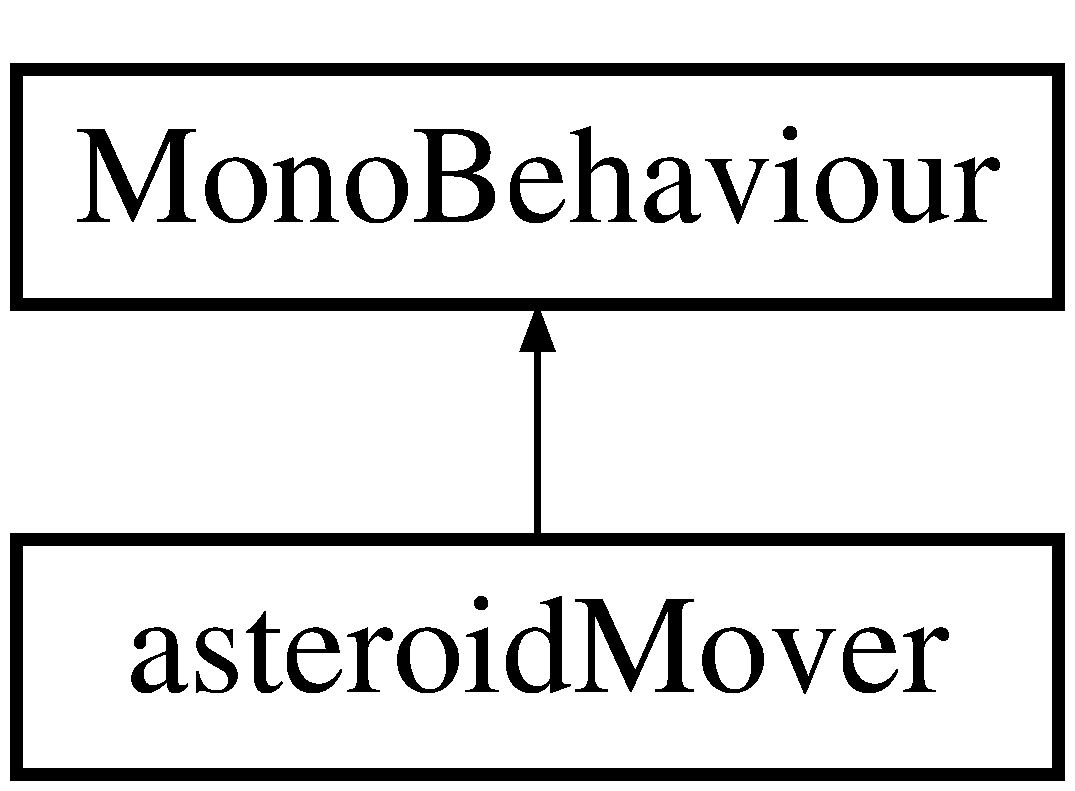
\includegraphics[height=2.000000cm]{classasteroid_mover}
\end{center}
\end{figure}
\subsection*{Private Member Functions}
\begin{DoxyCompactItemize}
\item 
void \mbox{\hyperlink{classasteroid_mover_a80e19d16f013e609127dfbdc53dbf817}{Start}} ()
\end{DoxyCompactItemize}
\subsection*{Private Attributes}
\begin{DoxyCompactItemize}
\item 
float \mbox{\hyperlink{classasteroid_mover_a1e23da1a73200fd4f129e5de86bdf32c}{speed}}
\end{DoxyCompactItemize}


\subsection{Member Function Documentation}
\mbox{\Hypertarget{classasteroid_mover_a80e19d16f013e609127dfbdc53dbf817}\label{classasteroid_mover_a80e19d16f013e609127dfbdc53dbf817}} 
\index{asteroid\+Mover@{asteroid\+Mover}!Start@{Start}}
\index{Start@{Start}!asteroid\+Mover@{asteroid\+Mover}}
\subsubsection{\texorpdfstring{Start()}{Start()}}
{\footnotesize\ttfamily void asteroid\+Mover.\+Start (\begin{DoxyParamCaption}{ }\end{DoxyParamCaption})\hspace{0.3cm}{\ttfamily [private]}}



\subsection{Member Data Documentation}
\mbox{\Hypertarget{classasteroid_mover_a1e23da1a73200fd4f129e5de86bdf32c}\label{classasteroid_mover_a1e23da1a73200fd4f129e5de86bdf32c}} 
\index{asteroid\+Mover@{asteroid\+Mover}!speed@{speed}}
\index{speed@{speed}!asteroid\+Mover@{asteroid\+Mover}}
\subsubsection{\texorpdfstring{speed}{speed}}
{\footnotesize\ttfamily float asteroid\+Mover.\+speed\hspace{0.3cm}{\ttfamily [private]}}



The documentation for this class was generated from the following file\+:\begin{DoxyCompactItemize}
\item 
\mbox{\hyperlink{asteroid_mover_8cs}{asteroid\+Mover.\+cs}}\end{DoxyCompactItemize}

\hypertarget{classasteroid_rotator}{}\section{asteroid\+Rotator Class Reference}
\label{classasteroid_rotator}\index{asteroid\+Rotator@{asteroid\+Rotator}}
Inheritance diagram for asteroid\+Rotator\+:\begin{figure}[H]
\begin{center}
\leavevmode
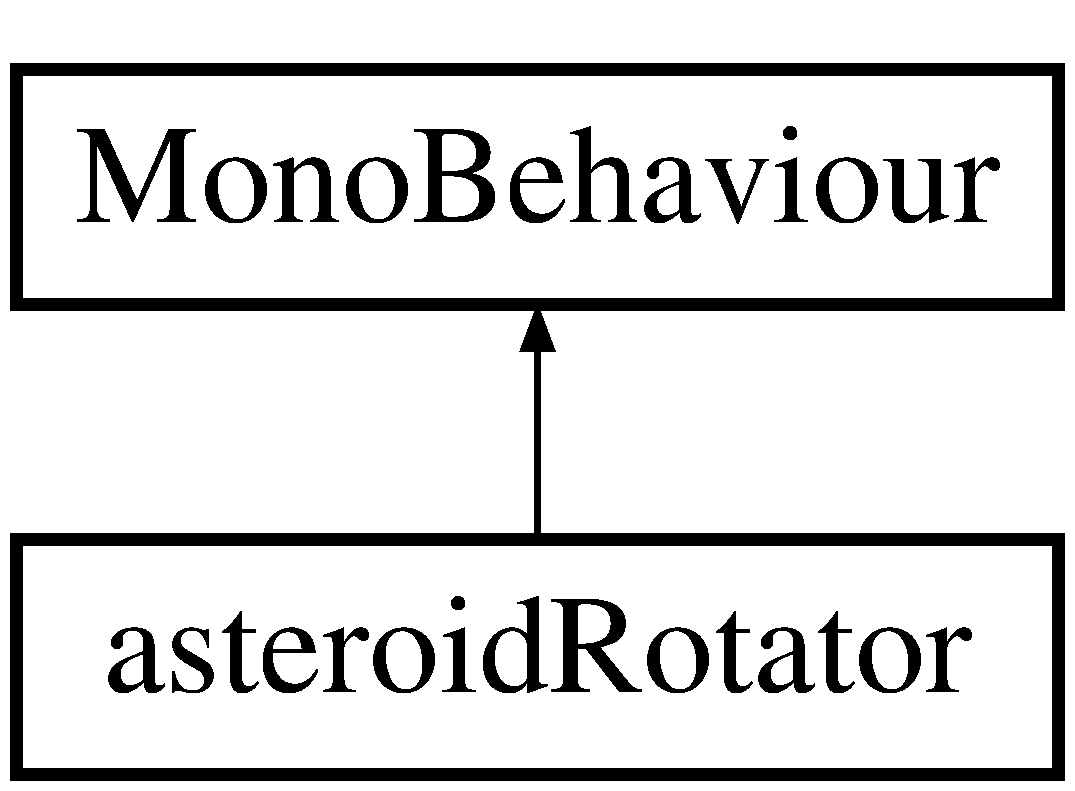
\includegraphics[height=2.000000cm]{classasteroid_rotator}
\end{center}
\end{figure}
\subsection*{Public Attributes}
\begin{DoxyCompactItemize}
\item 
float \mbox{\hyperlink{classasteroid_rotator_aa56366ba6b72b12f75b7dfaefc7fe7d6}{max\+Tumble}}
\end{DoxyCompactItemize}
\subsection*{Private Member Functions}
\begin{DoxyCompactItemize}
\item 
void \mbox{\hyperlink{classasteroid_rotator_a13e2d5d3e11fb68dc9b35f0e99c597c7}{Start}} ()
\end{DoxyCompactItemize}


\subsection{Member Function Documentation}
\mbox{\Hypertarget{classasteroid_rotator_a13e2d5d3e11fb68dc9b35f0e99c597c7}\label{classasteroid_rotator_a13e2d5d3e11fb68dc9b35f0e99c597c7}} 
\index{asteroid\+Rotator@{asteroid\+Rotator}!Start@{Start}}
\index{Start@{Start}!asteroid\+Rotator@{asteroid\+Rotator}}
\subsubsection{\texorpdfstring{Start()}{Start()}}
{\footnotesize\ttfamily void asteroid\+Rotator.\+Start (\begin{DoxyParamCaption}{ }\end{DoxyParamCaption})\hspace{0.3cm}{\ttfamily [private]}}



\subsection{Member Data Documentation}
\mbox{\Hypertarget{classasteroid_rotator_aa56366ba6b72b12f75b7dfaefc7fe7d6}\label{classasteroid_rotator_aa56366ba6b72b12f75b7dfaefc7fe7d6}} 
\index{asteroid\+Rotator@{asteroid\+Rotator}!max\+Tumble@{max\+Tumble}}
\index{max\+Tumble@{max\+Tumble}!asteroid\+Rotator@{asteroid\+Rotator}}
\subsubsection{\texorpdfstring{max\+Tumble}{maxTumble}}
{\footnotesize\ttfamily float asteroid\+Rotator.\+max\+Tumble}



The documentation for this class was generated from the following file\+:\begin{DoxyCompactItemize}
\item 
\mbox{\hyperlink{asteroid_rotator_8cs}{asteroid\+Rotator.\+cs}}\end{DoxyCompactItemize}

\hypertarget{class_b_g_scroller}{}\section{B\+G\+Scroller Class Reference}
\label{class_b_g_scroller}\index{B\+G\+Scroller@{B\+G\+Scroller}}
Inheritance diagram for B\+G\+Scroller\+:\begin{figure}[H]
\begin{center}
\leavevmode
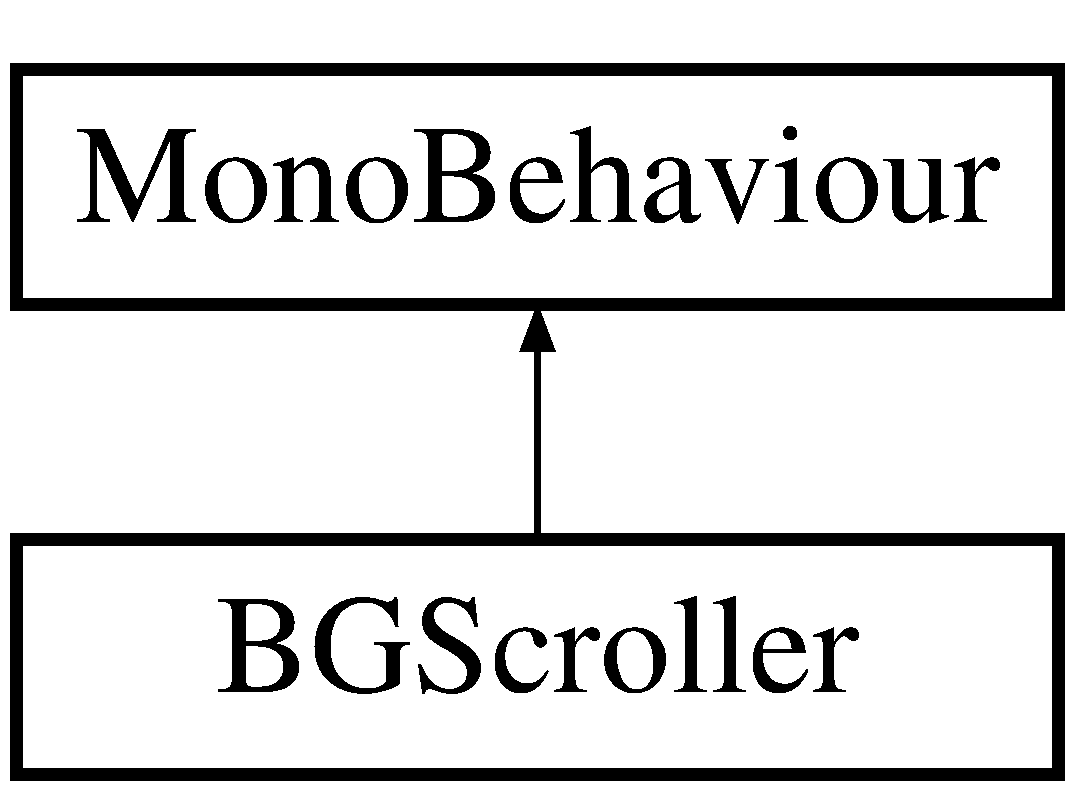
\includegraphics[height=2.000000cm]{class_b_g_scroller}
\end{center}
\end{figure}
\subsection*{Public Attributes}
\begin{DoxyCompactItemize}
\item 
float \mbox{\hyperlink{class_b_g_scroller_a31ae764c810451258f69c9e15def429f}{scroll\+Speed}}
\item 
float \mbox{\hyperlink{class_b_g_scroller_aa59f8685bd548c55d50c8396ae28ff2f}{tile\+SizeZ}}
\end{DoxyCompactItemize}
\subsection*{Private Member Functions}
\begin{DoxyCompactItemize}
\item 
void \mbox{\hyperlink{class_b_g_scroller_a7828067d39d4fe21cf4587dac494b59d}{Start}} ()
\item 
void \mbox{\hyperlink{class_b_g_scroller_a317fd0b2bb09e0ff6c281bd1be64c751}{Update}} ()
\end{DoxyCompactItemize}
\subsection*{Private Attributes}
\begin{DoxyCompactItemize}
\item 
Vector3 \mbox{\hyperlink{class_b_g_scroller_aeeaa39460879994b538440af714336d3}{start\+Position}}
\end{DoxyCompactItemize}


\subsection{Member Function Documentation}
\mbox{\Hypertarget{class_b_g_scroller_a7828067d39d4fe21cf4587dac494b59d}\label{class_b_g_scroller_a7828067d39d4fe21cf4587dac494b59d}} 
\index{B\+G\+Scroller@{B\+G\+Scroller}!Start@{Start}}
\index{Start@{Start}!B\+G\+Scroller@{B\+G\+Scroller}}
\subsubsection{\texorpdfstring{Start()}{Start()}}
{\footnotesize\ttfamily void B\+G\+Scroller.\+Start (\begin{DoxyParamCaption}{ }\end{DoxyParamCaption})\hspace{0.3cm}{\ttfamily [private]}}

\mbox{\Hypertarget{class_b_g_scroller_a317fd0b2bb09e0ff6c281bd1be64c751}\label{class_b_g_scroller_a317fd0b2bb09e0ff6c281bd1be64c751}} 
\index{B\+G\+Scroller@{B\+G\+Scroller}!Update@{Update}}
\index{Update@{Update}!B\+G\+Scroller@{B\+G\+Scroller}}
\subsubsection{\texorpdfstring{Update()}{Update()}}
{\footnotesize\ttfamily void B\+G\+Scroller.\+Update (\begin{DoxyParamCaption}{ }\end{DoxyParamCaption})\hspace{0.3cm}{\ttfamily [private]}}



\subsection{Member Data Documentation}
\mbox{\Hypertarget{class_b_g_scroller_a31ae764c810451258f69c9e15def429f}\label{class_b_g_scroller_a31ae764c810451258f69c9e15def429f}} 
\index{B\+G\+Scroller@{B\+G\+Scroller}!scroll\+Speed@{scroll\+Speed}}
\index{scroll\+Speed@{scroll\+Speed}!B\+G\+Scroller@{B\+G\+Scroller}}
\subsubsection{\texorpdfstring{scroll\+Speed}{scrollSpeed}}
{\footnotesize\ttfamily float B\+G\+Scroller.\+scroll\+Speed}

\mbox{\Hypertarget{class_b_g_scroller_aeeaa39460879994b538440af714336d3}\label{class_b_g_scroller_aeeaa39460879994b538440af714336d3}} 
\index{B\+G\+Scroller@{B\+G\+Scroller}!start\+Position@{start\+Position}}
\index{start\+Position@{start\+Position}!B\+G\+Scroller@{B\+G\+Scroller}}
\subsubsection{\texorpdfstring{start\+Position}{startPosition}}
{\footnotesize\ttfamily Vector3 B\+G\+Scroller.\+start\+Position\hspace{0.3cm}{\ttfamily [private]}}

\mbox{\Hypertarget{class_b_g_scroller_aa59f8685bd548c55d50c8396ae28ff2f}\label{class_b_g_scroller_aa59f8685bd548c55d50c8396ae28ff2f}} 
\index{B\+G\+Scroller@{B\+G\+Scroller}!tile\+SizeZ@{tile\+SizeZ}}
\index{tile\+SizeZ@{tile\+SizeZ}!B\+G\+Scroller@{B\+G\+Scroller}}
\subsubsection{\texorpdfstring{tile\+SizeZ}{tileSizeZ}}
{\footnotesize\ttfamily float B\+G\+Scroller.\+tile\+SizeZ}



The documentation for this class was generated from the following file\+:\begin{DoxyCompactItemize}
\item 
\mbox{\hyperlink{_b_g_scroller_8cs}{B\+G\+Scroller.\+cs}}\end{DoxyCompactItemize}

\hypertarget{classdestroy_asteroid}{}\section{destroy\+Asteroid Class Reference}
\label{classdestroy_asteroid}\index{destroy\+Asteroid@{destroy\+Asteroid}}
Inheritance diagram for destroy\+Asteroid\+:\begin{figure}[H]
\begin{center}
\leavevmode
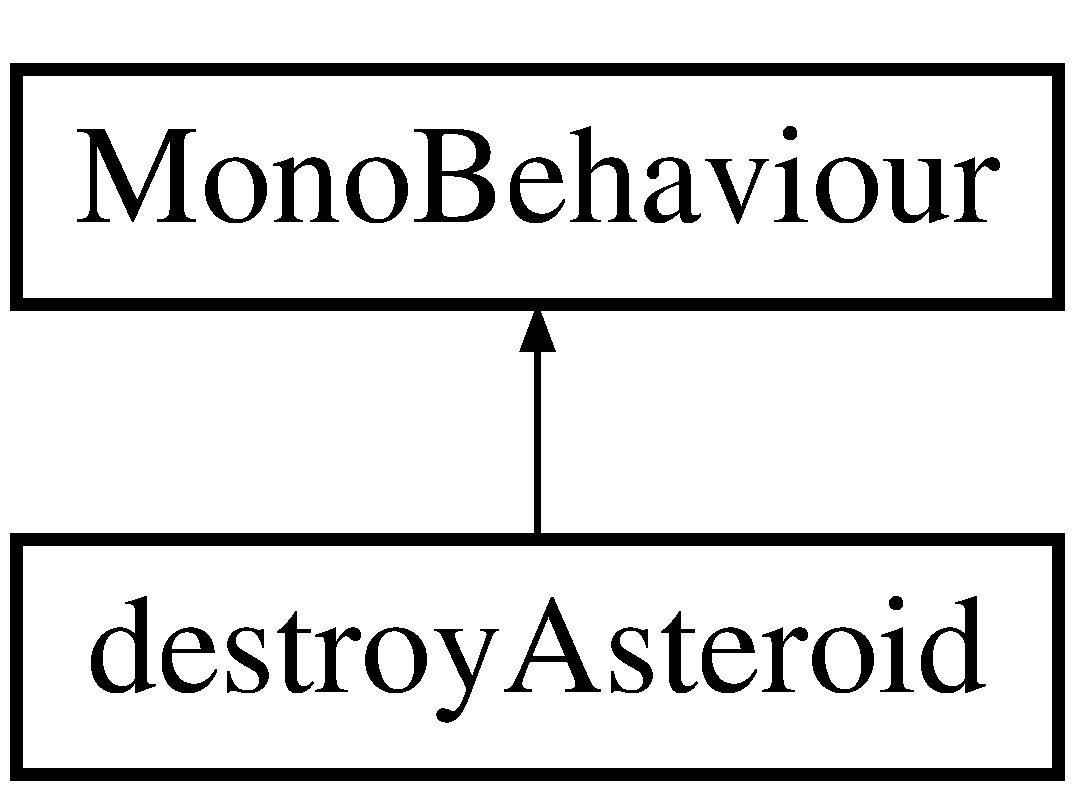
\includegraphics[height=2.000000cm]{classdestroy_asteroid}
\end{center}
\end{figure}
\subsection*{Public Attributes}
\begin{DoxyCompactItemize}
\item 
Game\+Object \mbox{\hyperlink{classdestroy_asteroid_a2018ced0016af9930b084fcd0925bf09}{explosion}}
\item 
Game\+Object \mbox{\hyperlink{classdestroy_asteroid_a965a9ae3de825dbd7aa7e1d178713305}{player\+Explosion}}
\end{DoxyCompactItemize}
\subsection*{Private Member Functions}
\begin{DoxyCompactItemize}
\item 
void \mbox{\hyperlink{classdestroy_asteroid_acb3ec8a3aa718e82ea7af340e7a4b1c4}{Start}} ()
\item 
void \mbox{\hyperlink{classdestroy_asteroid_ae4487b546e704cf723006a2acf5915a0}{On\+Trigger\+Enter}} (Collider other)
\end{DoxyCompactItemize}
\subsection*{Private Attributes}
\begin{DoxyCompactItemize}
\item 
int \mbox{\hyperlink{classdestroy_asteroid_ab3249e724efaf100a9ae754787ef0e6d}{score\+Value}} = 100
\item 
\mbox{\hyperlink{class_game_controller}{Game\+Controller}} \mbox{\hyperlink{classdestroy_asteroid_aefc18b1603f8dd4e4ece9dc65ec46a48}{game\+Controller}}
\end{DoxyCompactItemize}


\subsection{Member Function Documentation}
\mbox{\Hypertarget{classdestroy_asteroid_ae4487b546e704cf723006a2acf5915a0}\label{classdestroy_asteroid_ae4487b546e704cf723006a2acf5915a0}} 
\index{destroy\+Asteroid@{destroy\+Asteroid}!On\+Trigger\+Enter@{On\+Trigger\+Enter}}
\index{On\+Trigger\+Enter@{On\+Trigger\+Enter}!destroy\+Asteroid@{destroy\+Asteroid}}
\subsubsection{\texorpdfstring{On\+Trigger\+Enter()}{OnTriggerEnter()}}
{\footnotesize\ttfamily void destroy\+Asteroid.\+On\+Trigger\+Enter (\begin{DoxyParamCaption}\item[{Collider}]{other }\end{DoxyParamCaption})\hspace{0.3cm}{\ttfamily [private]}}

\mbox{\Hypertarget{classdestroy_asteroid_acb3ec8a3aa718e82ea7af340e7a4b1c4}\label{classdestroy_asteroid_acb3ec8a3aa718e82ea7af340e7a4b1c4}} 
\index{destroy\+Asteroid@{destroy\+Asteroid}!Start@{Start}}
\index{Start@{Start}!destroy\+Asteroid@{destroy\+Asteroid}}
\subsubsection{\texorpdfstring{Start()}{Start()}}
{\footnotesize\ttfamily void destroy\+Asteroid.\+Start (\begin{DoxyParamCaption}{ }\end{DoxyParamCaption})\hspace{0.3cm}{\ttfamily [private]}}



\subsection{Member Data Documentation}
\mbox{\Hypertarget{classdestroy_asteroid_a2018ced0016af9930b084fcd0925bf09}\label{classdestroy_asteroid_a2018ced0016af9930b084fcd0925bf09}} 
\index{destroy\+Asteroid@{destroy\+Asteroid}!explosion@{explosion}}
\index{explosion@{explosion}!destroy\+Asteroid@{destroy\+Asteroid}}
\subsubsection{\texorpdfstring{explosion}{explosion}}
{\footnotesize\ttfamily Game\+Object destroy\+Asteroid.\+explosion}

\mbox{\Hypertarget{classdestroy_asteroid_aefc18b1603f8dd4e4ece9dc65ec46a48}\label{classdestroy_asteroid_aefc18b1603f8dd4e4ece9dc65ec46a48}} 
\index{destroy\+Asteroid@{destroy\+Asteroid}!game\+Controller@{game\+Controller}}
\index{game\+Controller@{game\+Controller}!destroy\+Asteroid@{destroy\+Asteroid}}
\subsubsection{\texorpdfstring{game\+Controller}{gameController}}
{\footnotesize\ttfamily \mbox{\hyperlink{class_game_controller}{Game\+Controller}} destroy\+Asteroid.\+game\+Controller\hspace{0.3cm}{\ttfamily [private]}}

\mbox{\Hypertarget{classdestroy_asteroid_a965a9ae3de825dbd7aa7e1d178713305}\label{classdestroy_asteroid_a965a9ae3de825dbd7aa7e1d178713305}} 
\index{destroy\+Asteroid@{destroy\+Asteroid}!player\+Explosion@{player\+Explosion}}
\index{player\+Explosion@{player\+Explosion}!destroy\+Asteroid@{destroy\+Asteroid}}
\subsubsection{\texorpdfstring{player\+Explosion}{playerExplosion}}
{\footnotesize\ttfamily Game\+Object destroy\+Asteroid.\+player\+Explosion}

\mbox{\Hypertarget{classdestroy_asteroid_ab3249e724efaf100a9ae754787ef0e6d}\label{classdestroy_asteroid_ab3249e724efaf100a9ae754787ef0e6d}} 
\index{destroy\+Asteroid@{destroy\+Asteroid}!score\+Value@{score\+Value}}
\index{score\+Value@{score\+Value}!destroy\+Asteroid@{destroy\+Asteroid}}
\subsubsection{\texorpdfstring{score\+Value}{scoreValue}}
{\footnotesize\ttfamily int destroy\+Asteroid.\+score\+Value = 100\hspace{0.3cm}{\ttfamily [private]}}



The documentation for this class was generated from the following file\+:\begin{DoxyCompactItemize}
\item 
\mbox{\hyperlink{destroy_asteroid_8cs}{destroy\+Asteroid.\+cs}}\end{DoxyCompactItemize}

\hypertarget{classdestroyby_time}{}\section{destroyby\+Time Class Reference}
\label{classdestroyby_time}\index{destroyby\+Time@{destroyby\+Time}}
Inheritance diagram for destroyby\+Time\+:\begin{figure}[H]
\begin{center}
\leavevmode
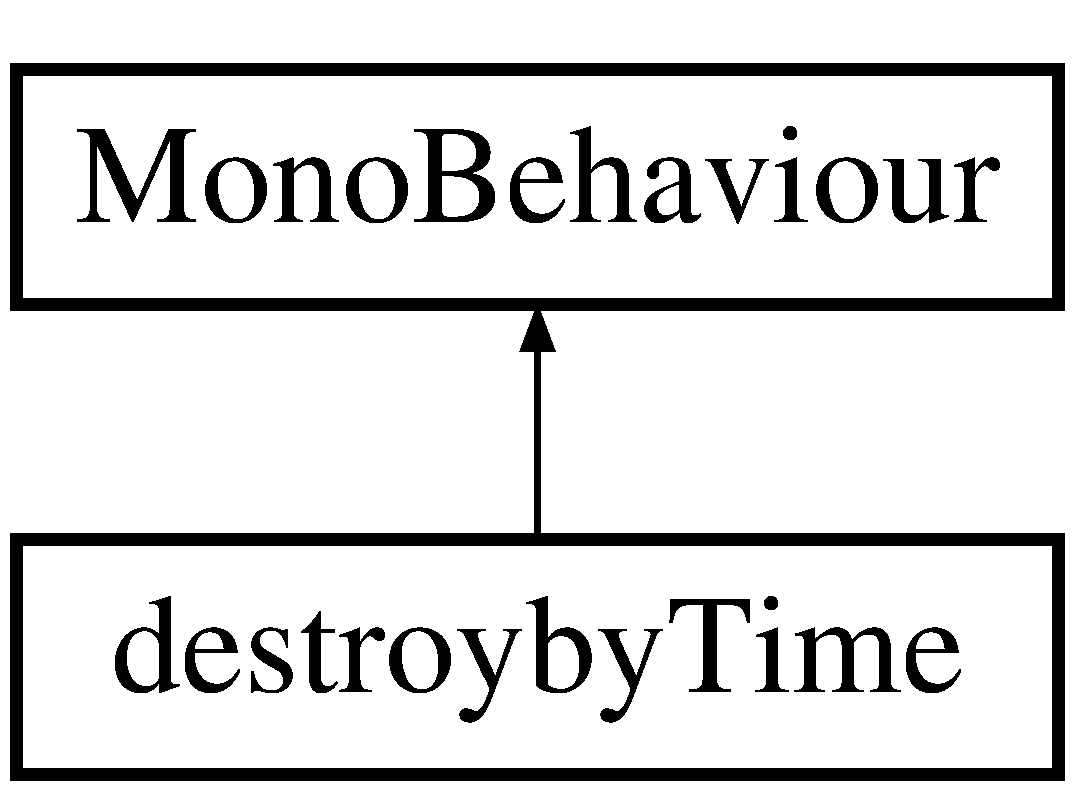
\includegraphics[height=2.000000cm]{classdestroyby_time}
\end{center}
\end{figure}
\subsection*{Public Attributes}
\begin{DoxyCompactItemize}
\item 
float \mbox{\hyperlink{classdestroyby_time_ad617cd8d5ba772f54506f8c897792cde}{lifetime}}
\end{DoxyCompactItemize}
\subsection*{Private Member Functions}
\begin{DoxyCompactItemize}
\item 
void \mbox{\hyperlink{classdestroyby_time_ad317df088f79babcc4e438e83d64ed66}{Start}} ()
\end{DoxyCompactItemize}


\subsection{Member Function Documentation}
\mbox{\Hypertarget{classdestroyby_time_ad317df088f79babcc4e438e83d64ed66}\label{classdestroyby_time_ad317df088f79babcc4e438e83d64ed66}} 
\index{destroyby\+Time@{destroyby\+Time}!Start@{Start}}
\index{Start@{Start}!destroyby\+Time@{destroyby\+Time}}
\subsubsection{\texorpdfstring{Start()}{Start()}}
{\footnotesize\ttfamily void destroyby\+Time.\+Start (\begin{DoxyParamCaption}{ }\end{DoxyParamCaption})\hspace{0.3cm}{\ttfamily [private]}}



\subsection{Member Data Documentation}
\mbox{\Hypertarget{classdestroyby_time_ad617cd8d5ba772f54506f8c897792cde}\label{classdestroyby_time_ad617cd8d5ba772f54506f8c897792cde}} 
\index{destroyby\+Time@{destroyby\+Time}!lifetime@{lifetime}}
\index{lifetime@{lifetime}!destroyby\+Time@{destroyby\+Time}}
\subsubsection{\texorpdfstring{lifetime}{lifetime}}
{\footnotesize\ttfamily float destroyby\+Time.\+lifetime}



The documentation for this class was generated from the following file\+:\begin{DoxyCompactItemize}
\item 
\mbox{\hyperlink{destroyby_time_8cs}{destroyby\+Time.\+cs}}\end{DoxyCompactItemize}

\hypertarget{class_game_controller}{}\section{Game\+Controller Class Reference}
\label{class_game_controller}\index{Game\+Controller@{Game\+Controller}}
Inheritance diagram for Game\+Controller\+:\begin{figure}[H]
\begin{center}
\leavevmode
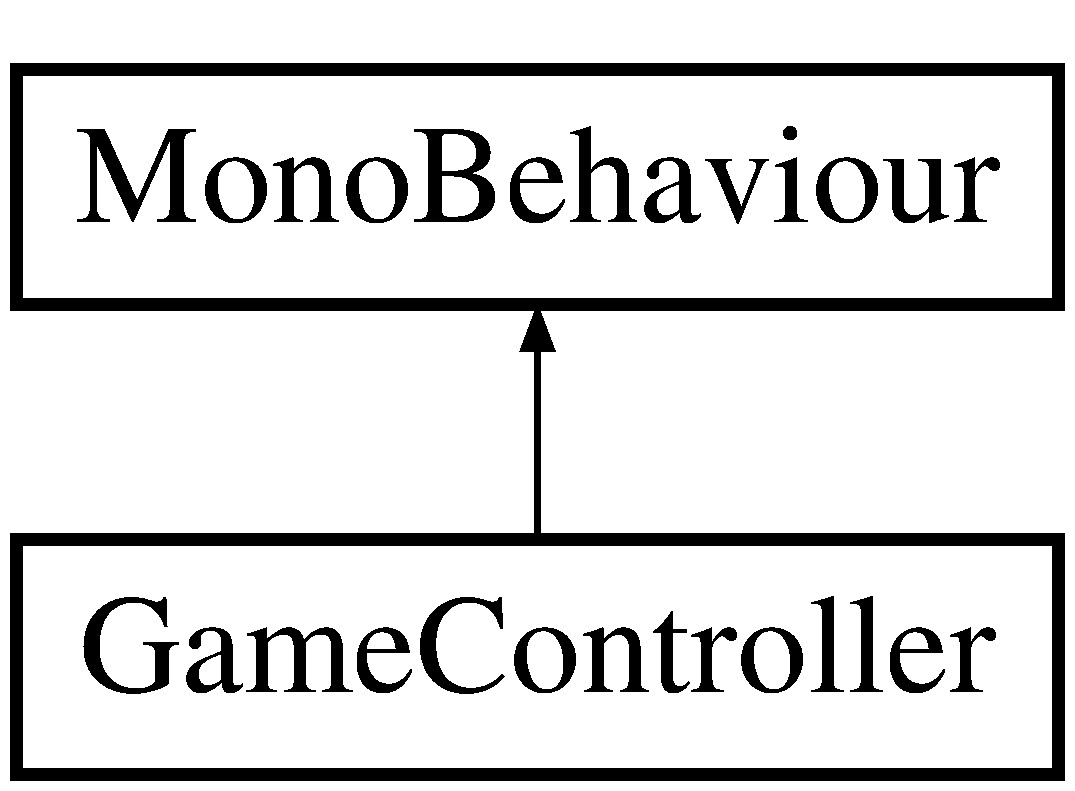
\includegraphics[height=2.000000cm]{class_game_controller}
\end{center}
\end{figure}
\subsection*{Public Member Functions}
\begin{DoxyCompactItemize}
\item 
void \mbox{\hyperlink{class_game_controller_a9cd49518487a342b5f635537d10b3589}{add\+Score}} (int new\+Score\+Value)
\item 
void \mbox{\hyperlink{class_game_controller_a867b359e465ba013eec7f1ee03b75118}{Game\+Over}} ()
\end{DoxyCompactItemize}
\subsection*{Public Attributes}
\begin{DoxyCompactItemize}
\item 
Game\+Object \mbox{\hyperlink{class_game_controller_ab280da3f329b7e2532dda6062a58f4fb}{asteroid}}
\item 
Vector3 \mbox{\hyperlink{class_game_controller_a5e4f56c23896d4b528da579f93335896}{spawn\+Values}}
\item 
int \mbox{\hyperlink{class_game_controller_aca9ea9aa49e5af784896d6b895f6be90}{asteroid\+Count}}
\item 
float \mbox{\hyperlink{class_game_controller_a27c91a14de3982813ad3d8245d0134d7}{spawn\+Wait}}
\item 
float \mbox{\hyperlink{class_game_controller_a9b6f96c29d3ee0f2c692c30ed2b12835}{start\+Wait}}
\item 
float \mbox{\hyperlink{class_game_controller_ad210270b367c1c439d35e8177d989019}{wave\+Wait}}
\item 
Text \mbox{\hyperlink{class_game_controller_ad59d43bc8b212847eaae1e877d8c1a31}{score\+Text}}
\item 
Text \mbox{\hyperlink{class_game_controller_aba4351ee1c41d1af6c44c2cb106a4b67}{game\+Over\+Text}}
\item 
Text \mbox{\hyperlink{class_game_controller_a68dea27fd0de9061889d2664697af64f}{restart\+Text}}
\end{DoxyCompactItemize}
\subsection*{Private Member Functions}
\begin{DoxyCompactItemize}
\item 
void \mbox{\hyperlink{class_game_controller_a97788a7aa0f09c8d748781683e5f045b}{Start}} ()
\item 
void \mbox{\hyperlink{class_game_controller_a5a89277529cadb49af7d55eba3bbf056}{Update}} ()
\item 
I\+Enumerator \mbox{\hyperlink{class_game_controller_afcbbff33b0d0fb1fed262dd67d52e9c3}{spawn\+Waves}} ()
\item 
void \mbox{\hyperlink{class_game_controller_a54d9efcafca6d05c967e375066ca1a27}{update\+Score}} ()
\end{DoxyCompactItemize}
\subsection*{Private Attributes}
\begin{DoxyCompactItemize}
\item 
float \mbox{\hyperlink{class_game_controller_aa8d3b5308427f0cbbbe8f34d3fd96d31}{difficulty}} = 0.\+0017f
\item 
int \mbox{\hyperlink{class_game_controller_a5262f16a935aa930f813ff9c0dc060f2}{score}}
\item 
bool \mbox{\hyperlink{class_game_controller_aeea923e78ddd573296687317e638a937}{restart}}
\item 
bool \mbox{\hyperlink{class_game_controller_aeae400ea0c604655ce5801818a5a44a1}{game\+Over}}
\end{DoxyCompactItemize}


\subsection{Member Function Documentation}
\mbox{\Hypertarget{class_game_controller_a9cd49518487a342b5f635537d10b3589}\label{class_game_controller_a9cd49518487a342b5f635537d10b3589}} 
\index{Game\+Controller@{Game\+Controller}!add\+Score@{add\+Score}}
\index{add\+Score@{add\+Score}!Game\+Controller@{Game\+Controller}}
\subsubsection{\texorpdfstring{add\+Score()}{addScore()}}
{\footnotesize\ttfamily void Game\+Controller.\+add\+Score (\begin{DoxyParamCaption}\item[{int}]{new\+Score\+Value }\end{DoxyParamCaption})}

\mbox{\Hypertarget{class_game_controller_a867b359e465ba013eec7f1ee03b75118}\label{class_game_controller_a867b359e465ba013eec7f1ee03b75118}} 
\index{Game\+Controller@{Game\+Controller}!Game\+Over@{Game\+Over}}
\index{Game\+Over@{Game\+Over}!Game\+Controller@{Game\+Controller}}
\subsubsection{\texorpdfstring{Game\+Over()}{GameOver()}}
{\footnotesize\ttfamily void Game\+Controller.\+Game\+Over (\begin{DoxyParamCaption}{ }\end{DoxyParamCaption})}

\mbox{\Hypertarget{class_game_controller_afcbbff33b0d0fb1fed262dd67d52e9c3}\label{class_game_controller_afcbbff33b0d0fb1fed262dd67d52e9c3}} 
\index{Game\+Controller@{Game\+Controller}!spawn\+Waves@{spawn\+Waves}}
\index{spawn\+Waves@{spawn\+Waves}!Game\+Controller@{Game\+Controller}}
\subsubsection{\texorpdfstring{spawn\+Waves()}{spawnWaves()}}
{\footnotesize\ttfamily I\+Enumerator Game\+Controller.\+spawn\+Waves (\begin{DoxyParamCaption}{ }\end{DoxyParamCaption})\hspace{0.3cm}{\ttfamily [private]}}

\mbox{\Hypertarget{class_game_controller_a97788a7aa0f09c8d748781683e5f045b}\label{class_game_controller_a97788a7aa0f09c8d748781683e5f045b}} 
\index{Game\+Controller@{Game\+Controller}!Start@{Start}}
\index{Start@{Start}!Game\+Controller@{Game\+Controller}}
\subsubsection{\texorpdfstring{Start()}{Start()}}
{\footnotesize\ttfamily void Game\+Controller.\+Start (\begin{DoxyParamCaption}{ }\end{DoxyParamCaption})\hspace{0.3cm}{\ttfamily [private]}}

\mbox{\Hypertarget{class_game_controller_a5a89277529cadb49af7d55eba3bbf056}\label{class_game_controller_a5a89277529cadb49af7d55eba3bbf056}} 
\index{Game\+Controller@{Game\+Controller}!Update@{Update}}
\index{Update@{Update}!Game\+Controller@{Game\+Controller}}
\subsubsection{\texorpdfstring{Update()}{Update()}}
{\footnotesize\ttfamily void Game\+Controller.\+Update (\begin{DoxyParamCaption}{ }\end{DoxyParamCaption})\hspace{0.3cm}{\ttfamily [private]}}

\mbox{\Hypertarget{class_game_controller_a54d9efcafca6d05c967e375066ca1a27}\label{class_game_controller_a54d9efcafca6d05c967e375066ca1a27}} 
\index{Game\+Controller@{Game\+Controller}!update\+Score@{update\+Score}}
\index{update\+Score@{update\+Score}!Game\+Controller@{Game\+Controller}}
\subsubsection{\texorpdfstring{update\+Score()}{updateScore()}}
{\footnotesize\ttfamily void Game\+Controller.\+update\+Score (\begin{DoxyParamCaption}{ }\end{DoxyParamCaption})\hspace{0.3cm}{\ttfamily [private]}}



\subsection{Member Data Documentation}
\mbox{\Hypertarget{class_game_controller_ab280da3f329b7e2532dda6062a58f4fb}\label{class_game_controller_ab280da3f329b7e2532dda6062a58f4fb}} 
\index{Game\+Controller@{Game\+Controller}!asteroid@{asteroid}}
\index{asteroid@{asteroid}!Game\+Controller@{Game\+Controller}}
\subsubsection{\texorpdfstring{asteroid}{asteroid}}
{\footnotesize\ttfamily Game\+Object Game\+Controller.\+asteroid}

\mbox{\Hypertarget{class_game_controller_aca9ea9aa49e5af784896d6b895f6be90}\label{class_game_controller_aca9ea9aa49e5af784896d6b895f6be90}} 
\index{Game\+Controller@{Game\+Controller}!asteroid\+Count@{asteroid\+Count}}
\index{asteroid\+Count@{asteroid\+Count}!Game\+Controller@{Game\+Controller}}
\subsubsection{\texorpdfstring{asteroid\+Count}{asteroidCount}}
{\footnotesize\ttfamily int Game\+Controller.\+asteroid\+Count}

\mbox{\Hypertarget{class_game_controller_aa8d3b5308427f0cbbbe8f34d3fd96d31}\label{class_game_controller_aa8d3b5308427f0cbbbe8f34d3fd96d31}} 
\index{Game\+Controller@{Game\+Controller}!difficulty@{difficulty}}
\index{difficulty@{difficulty}!Game\+Controller@{Game\+Controller}}
\subsubsection{\texorpdfstring{difficulty}{difficulty}}
{\footnotesize\ttfamily float Game\+Controller.\+difficulty = 0.\+0017f\hspace{0.3cm}{\ttfamily [private]}}

\mbox{\Hypertarget{class_game_controller_aeae400ea0c604655ce5801818a5a44a1}\label{class_game_controller_aeae400ea0c604655ce5801818a5a44a1}} 
\index{Game\+Controller@{Game\+Controller}!game\+Over@{game\+Over}}
\index{game\+Over@{game\+Over}!Game\+Controller@{Game\+Controller}}
\subsubsection{\texorpdfstring{game\+Over}{gameOver}}
{\footnotesize\ttfamily bool Game\+Controller.\+game\+Over\hspace{0.3cm}{\ttfamily [private]}}

\mbox{\Hypertarget{class_game_controller_aba4351ee1c41d1af6c44c2cb106a4b67}\label{class_game_controller_aba4351ee1c41d1af6c44c2cb106a4b67}} 
\index{Game\+Controller@{Game\+Controller}!game\+Over\+Text@{game\+Over\+Text}}
\index{game\+Over\+Text@{game\+Over\+Text}!Game\+Controller@{Game\+Controller}}
\subsubsection{\texorpdfstring{game\+Over\+Text}{gameOverText}}
{\footnotesize\ttfamily Text Game\+Controller.\+game\+Over\+Text}

\mbox{\Hypertarget{class_game_controller_aeea923e78ddd573296687317e638a937}\label{class_game_controller_aeea923e78ddd573296687317e638a937}} 
\index{Game\+Controller@{Game\+Controller}!restart@{restart}}
\index{restart@{restart}!Game\+Controller@{Game\+Controller}}
\subsubsection{\texorpdfstring{restart}{restart}}
{\footnotesize\ttfamily bool Game\+Controller.\+restart\hspace{0.3cm}{\ttfamily [private]}}

\mbox{\Hypertarget{class_game_controller_a68dea27fd0de9061889d2664697af64f}\label{class_game_controller_a68dea27fd0de9061889d2664697af64f}} 
\index{Game\+Controller@{Game\+Controller}!restart\+Text@{restart\+Text}}
\index{restart\+Text@{restart\+Text}!Game\+Controller@{Game\+Controller}}
\subsubsection{\texorpdfstring{restart\+Text}{restartText}}
{\footnotesize\ttfamily Text Game\+Controller.\+restart\+Text}

\mbox{\Hypertarget{class_game_controller_a5262f16a935aa930f813ff9c0dc060f2}\label{class_game_controller_a5262f16a935aa930f813ff9c0dc060f2}} 
\index{Game\+Controller@{Game\+Controller}!score@{score}}
\index{score@{score}!Game\+Controller@{Game\+Controller}}
\subsubsection{\texorpdfstring{score}{score}}
{\footnotesize\ttfamily int Game\+Controller.\+score\hspace{0.3cm}{\ttfamily [private]}}

\mbox{\Hypertarget{class_game_controller_ad59d43bc8b212847eaae1e877d8c1a31}\label{class_game_controller_ad59d43bc8b212847eaae1e877d8c1a31}} 
\index{Game\+Controller@{Game\+Controller}!score\+Text@{score\+Text}}
\index{score\+Text@{score\+Text}!Game\+Controller@{Game\+Controller}}
\subsubsection{\texorpdfstring{score\+Text}{scoreText}}
{\footnotesize\ttfamily Text Game\+Controller.\+score\+Text}

\mbox{\Hypertarget{class_game_controller_a5e4f56c23896d4b528da579f93335896}\label{class_game_controller_a5e4f56c23896d4b528da579f93335896}} 
\index{Game\+Controller@{Game\+Controller}!spawn\+Values@{spawn\+Values}}
\index{spawn\+Values@{spawn\+Values}!Game\+Controller@{Game\+Controller}}
\subsubsection{\texorpdfstring{spawn\+Values}{spawnValues}}
{\footnotesize\ttfamily Vector3 Game\+Controller.\+spawn\+Values}

\mbox{\Hypertarget{class_game_controller_a27c91a14de3982813ad3d8245d0134d7}\label{class_game_controller_a27c91a14de3982813ad3d8245d0134d7}} 
\index{Game\+Controller@{Game\+Controller}!spawn\+Wait@{spawn\+Wait}}
\index{spawn\+Wait@{spawn\+Wait}!Game\+Controller@{Game\+Controller}}
\subsubsection{\texorpdfstring{spawn\+Wait}{spawnWait}}
{\footnotesize\ttfamily float Game\+Controller.\+spawn\+Wait}

\mbox{\Hypertarget{class_game_controller_a9b6f96c29d3ee0f2c692c30ed2b12835}\label{class_game_controller_a9b6f96c29d3ee0f2c692c30ed2b12835}} 
\index{Game\+Controller@{Game\+Controller}!start\+Wait@{start\+Wait}}
\index{start\+Wait@{start\+Wait}!Game\+Controller@{Game\+Controller}}
\subsubsection{\texorpdfstring{start\+Wait}{startWait}}
{\footnotesize\ttfamily float Game\+Controller.\+start\+Wait}

\mbox{\Hypertarget{class_game_controller_ad210270b367c1c439d35e8177d989019}\label{class_game_controller_ad210270b367c1c439d35e8177d989019}} 
\index{Game\+Controller@{Game\+Controller}!wave\+Wait@{wave\+Wait}}
\index{wave\+Wait@{wave\+Wait}!Game\+Controller@{Game\+Controller}}
\subsubsection{\texorpdfstring{wave\+Wait}{waveWait}}
{\footnotesize\ttfamily float Game\+Controller.\+wave\+Wait}



The documentation for this class was generated from the following file\+:\begin{DoxyCompactItemize}
\item 
\mbox{\hyperlink{_game_controller_8cs}{Game\+Controller.\+cs}}\end{DoxyCompactItemize}

\hypertarget{classlaser_movement}{}\section{laser\+Movement Class Reference}
\label{classlaser_movement}\index{laser\+Movement@{laser\+Movement}}
Inheritance diagram for laser\+Movement\+:\begin{figure}[H]
\begin{center}
\leavevmode
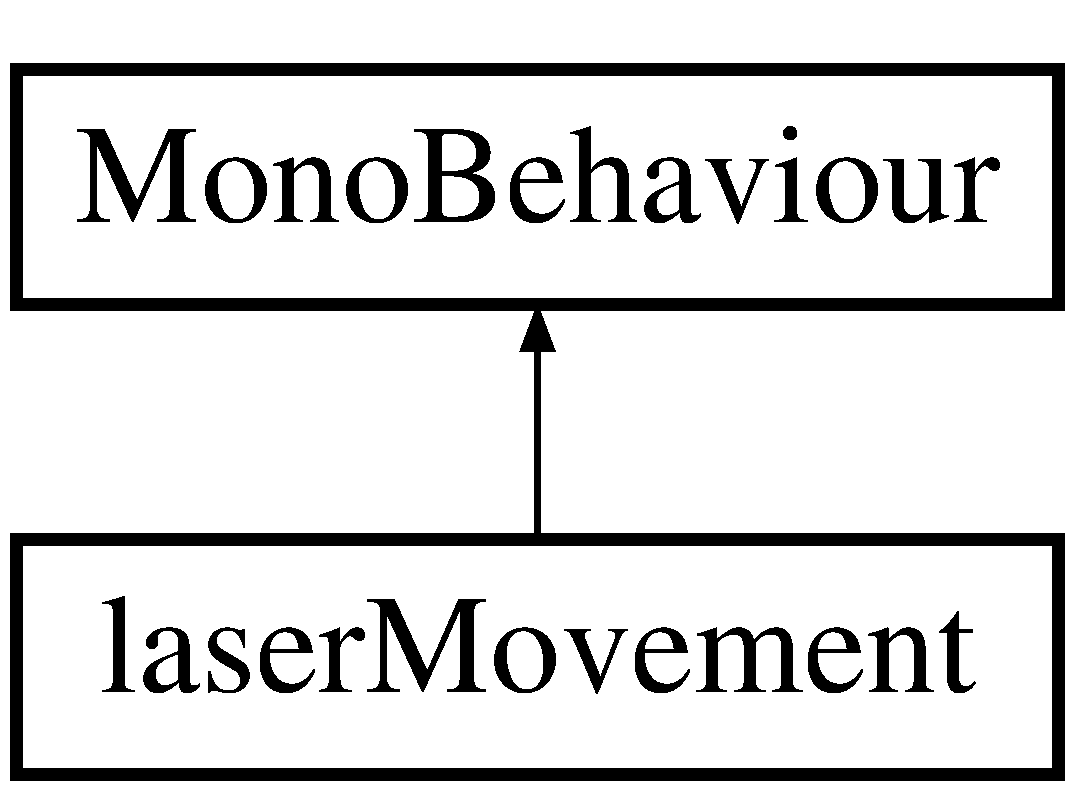
\includegraphics[height=2.000000cm]{classlaser_movement}
\end{center}
\end{figure}
\subsection*{Public Attributes}
\begin{DoxyCompactItemize}
\item 
float \mbox{\hyperlink{classlaser_movement_a970c3ffad1f10386b83d4f54dcebc21d}{speed}}
\end{DoxyCompactItemize}
\subsection*{Private Member Functions}
\begin{DoxyCompactItemize}
\item 
void \mbox{\hyperlink{classlaser_movement_aaa5cabcbfc82ac37257730af9b842f7f}{Start}} ()
\end{DoxyCompactItemize}
\subsection*{Private Attributes}
\begin{DoxyCompactItemize}
\item 
Rigidbody \mbox{\hyperlink{classlaser_movement_ae7c67c229eb3081c017be2f359db80e3}{laser\+Comp}}
\end{DoxyCompactItemize}


\subsection{Member Function Documentation}
\mbox{\Hypertarget{classlaser_movement_aaa5cabcbfc82ac37257730af9b842f7f}\label{classlaser_movement_aaa5cabcbfc82ac37257730af9b842f7f}} 
\index{laser\+Movement@{laser\+Movement}!Start@{Start}}
\index{Start@{Start}!laser\+Movement@{laser\+Movement}}
\subsubsection{\texorpdfstring{Start()}{Start()}}
{\footnotesize\ttfamily void laser\+Movement.\+Start (\begin{DoxyParamCaption}{ }\end{DoxyParamCaption})\hspace{0.3cm}{\ttfamily [private]}}



\subsection{Member Data Documentation}
\mbox{\Hypertarget{classlaser_movement_ae7c67c229eb3081c017be2f359db80e3}\label{classlaser_movement_ae7c67c229eb3081c017be2f359db80e3}} 
\index{laser\+Movement@{laser\+Movement}!laser\+Comp@{laser\+Comp}}
\index{laser\+Comp@{laser\+Comp}!laser\+Movement@{laser\+Movement}}
\subsubsection{\texorpdfstring{laser\+Comp}{laserComp}}
{\footnotesize\ttfamily Rigidbody laser\+Movement.\+laser\+Comp\hspace{0.3cm}{\ttfamily [private]}}

\mbox{\Hypertarget{classlaser_movement_a970c3ffad1f10386b83d4f54dcebc21d}\label{classlaser_movement_a970c3ffad1f10386b83d4f54dcebc21d}} 
\index{laser\+Movement@{laser\+Movement}!speed@{speed}}
\index{speed@{speed}!laser\+Movement@{laser\+Movement}}
\subsubsection{\texorpdfstring{speed}{speed}}
{\footnotesize\ttfamily float laser\+Movement.\+speed}



The documentation for this class was generated from the following file\+:\begin{DoxyCompactItemize}
\item 
\mbox{\hyperlink{laser_movement_8cs}{laser\+Movement.\+cs}}\end{DoxyCompactItemize}

\hypertarget{class_map_bounds}{}\section{Map\+Bounds Class Reference}
\label{class_map_bounds}\index{Map\+Bounds@{Map\+Bounds}}
\subsection*{Public Attributes}
\begin{DoxyCompactItemize}
\item 
float \mbox{\hyperlink{class_map_bounds_a00d303898481a2216ef8aa6101788201}{x\+Min}}
\end{DoxyCompactItemize}
\subsection*{Private Attributes}
\begin{DoxyCompactItemize}
\item 
float \mbox{\hyperlink{class_map_bounds_a072bf7a7bd172ae41b05799223e52550}{x\+Max}}
\item 
float \mbox{\hyperlink{class_map_bounds_a10c2fbda66927f1d51dab5ac2f396b0f}{z\+Min}}
\item 
float \mbox{\hyperlink{class_map_bounds_ade583e88139ad09d8f232052c5ee2fd0}{z\+Max}}
\end{DoxyCompactItemize}


\subsection{Member Data Documentation}
\mbox{\Hypertarget{class_map_bounds_a072bf7a7bd172ae41b05799223e52550}\label{class_map_bounds_a072bf7a7bd172ae41b05799223e52550}} 
\index{Map\+Bounds@{Map\+Bounds}!x\+Max@{x\+Max}}
\index{x\+Max@{x\+Max}!Map\+Bounds@{Map\+Bounds}}
\subsubsection{\texorpdfstring{x\+Max}{xMax}}
{\footnotesize\ttfamily float Map\+Bounds.\+x\+Max\hspace{0.3cm}{\ttfamily [private]}}

\mbox{\Hypertarget{class_map_bounds_a00d303898481a2216ef8aa6101788201}\label{class_map_bounds_a00d303898481a2216ef8aa6101788201}} 
\index{Map\+Bounds@{Map\+Bounds}!x\+Min@{x\+Min}}
\index{x\+Min@{x\+Min}!Map\+Bounds@{Map\+Bounds}}
\subsubsection{\texorpdfstring{x\+Min}{xMin}}
{\footnotesize\ttfamily float Map\+Bounds.\+x\+Min}

\mbox{\Hypertarget{class_map_bounds_ade583e88139ad09d8f232052c5ee2fd0}\label{class_map_bounds_ade583e88139ad09d8f232052c5ee2fd0}} 
\index{Map\+Bounds@{Map\+Bounds}!z\+Max@{z\+Max}}
\index{z\+Max@{z\+Max}!Map\+Bounds@{Map\+Bounds}}
\subsubsection{\texorpdfstring{z\+Max}{zMax}}
{\footnotesize\ttfamily float Map\+Bounds.\+z\+Max\hspace{0.3cm}{\ttfamily [private]}}

\mbox{\Hypertarget{class_map_bounds_a10c2fbda66927f1d51dab5ac2f396b0f}\label{class_map_bounds_a10c2fbda66927f1d51dab5ac2f396b0f}} 
\index{Map\+Bounds@{Map\+Bounds}!z\+Min@{z\+Min}}
\index{z\+Min@{z\+Min}!Map\+Bounds@{Map\+Bounds}}
\subsubsection{\texorpdfstring{z\+Min}{zMin}}
{\footnotesize\ttfamily float Map\+Bounds.\+z\+Min\hspace{0.3cm}{\ttfamily [private]}}



The documentation for this class was generated from the following file\+:\begin{DoxyCompactItemize}
\item 
\mbox{\hyperlink{_player_controller_8cs}{Player\+Controller.\+cs}}\end{DoxyCompactItemize}

\hypertarget{classout_of_bounds}{}\section{out\+Of\+Bounds Class Reference}
\label{classout_of_bounds}\index{out\+Of\+Bounds@{out\+Of\+Bounds}}
Inheritance diagram for out\+Of\+Bounds\+:\begin{figure}[H]
\begin{center}
\leavevmode
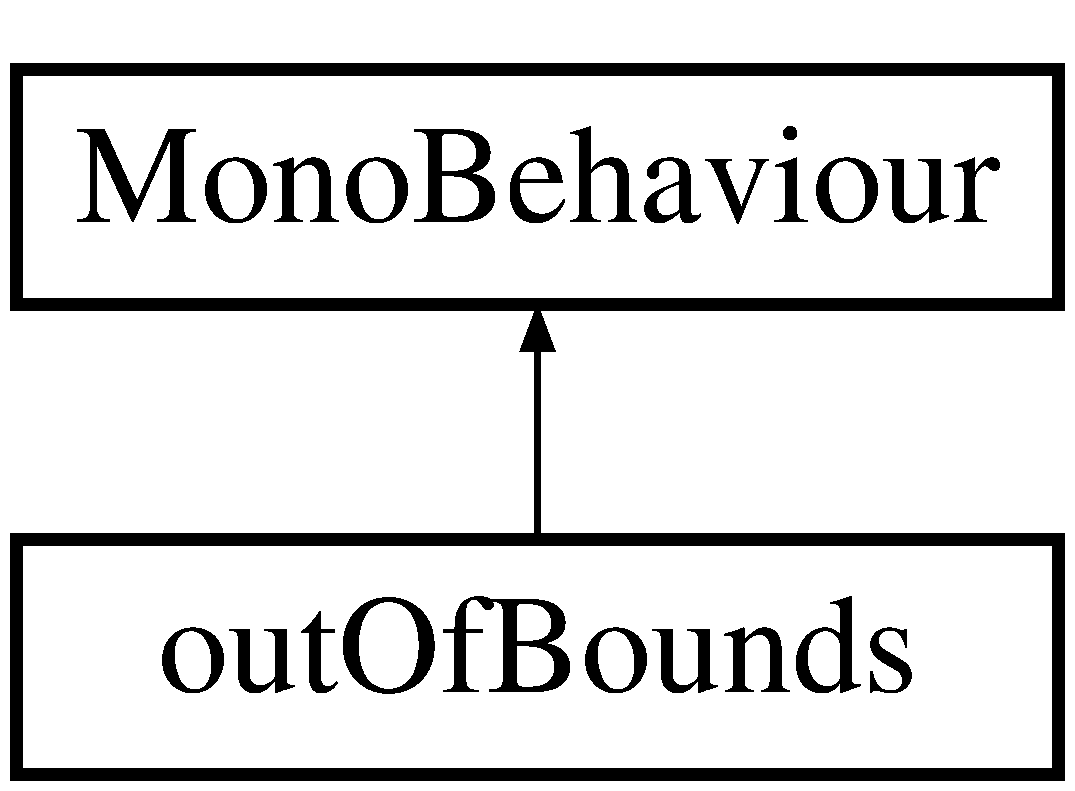
\includegraphics[height=2.000000cm]{classout_of_bounds}
\end{center}
\end{figure}
\subsection*{Private Member Functions}
\begin{DoxyCompactItemize}
\item 
void \mbox{\hyperlink{classout_of_bounds_ae4f37639924e582f648b5caa8d8cc448}{On\+Trigger\+Exit}} (Collider other)
\end{DoxyCompactItemize}


\subsection{Member Function Documentation}
\mbox{\Hypertarget{classout_of_bounds_ae4f37639924e582f648b5caa8d8cc448}\label{classout_of_bounds_ae4f37639924e582f648b5caa8d8cc448}} 
\index{out\+Of\+Bounds@{out\+Of\+Bounds}!On\+Trigger\+Exit@{On\+Trigger\+Exit}}
\index{On\+Trigger\+Exit@{On\+Trigger\+Exit}!out\+Of\+Bounds@{out\+Of\+Bounds}}
\subsubsection{\texorpdfstring{On\+Trigger\+Exit()}{OnTriggerExit()}}
{\footnotesize\ttfamily void out\+Of\+Bounds.\+On\+Trigger\+Exit (\begin{DoxyParamCaption}\item[{Collider}]{other }\end{DoxyParamCaption})\hspace{0.3cm}{\ttfamily [private]}}



The documentation for this class was generated from the following file\+:\begin{DoxyCompactItemize}
\item 
\mbox{\hyperlink{out_of_bounds_8cs}{out\+Of\+Bounds.\+cs}}\end{DoxyCompactItemize}

\hypertarget{class_player_controller}{}\section{Player\+Controller Class Reference}
\label{class_player_controller}\index{Player\+Controller@{Player\+Controller}}
Inheritance diagram for Player\+Controller\+:\begin{figure}[H]
\begin{center}
\leavevmode
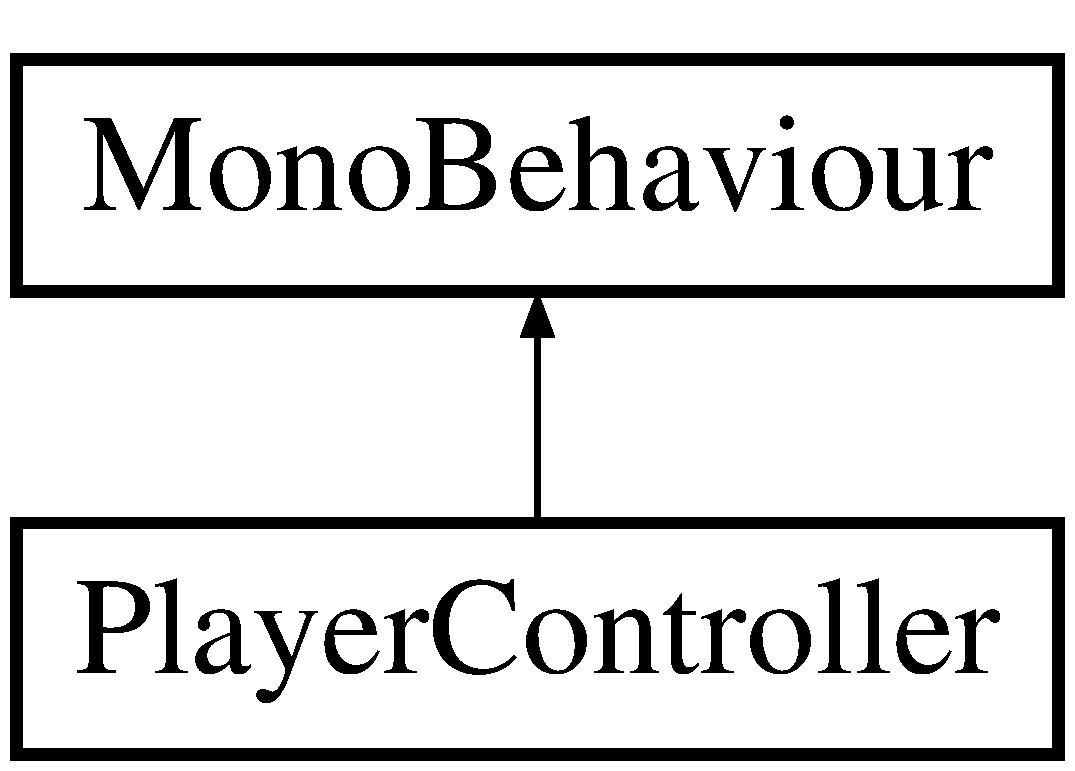
\includegraphics[height=2.000000cm]{class_player_controller}
\end{center}
\end{figure}
\subsection*{Public Attributes}
\begin{DoxyCompactItemize}
\item 
\mbox{\hyperlink{class_map_bounds}{Map\+Bounds}} \mbox{\hyperlink{class_player_controller_ae7832037e53c9031202ad60873a11498}{map}}
\item 
Game\+Object \mbox{\hyperlink{class_player_controller_a690a962b91653c2fdba718d5775a60eb}{Laser}}
\item 
Transform \mbox{\hyperlink{class_player_controller_ad0643bd4ceef85ae7e427bd08a7fd401}{start\+Laser}}
\item 
float \mbox{\hyperlink{class_player_controller_a0928605583f0563cd84fe43119d336ec}{speed}}
\item 
float \mbox{\hyperlink{class_player_controller_ac3e62babe8d87ccdfc0216fac5fe1688}{tilt}}
\item 
float \mbox{\hyperlink{class_player_controller_aec1e8f25c69ea198fe38f965307437a4}{fire\+Rate}}
\end{DoxyCompactItemize}
\subsection*{Private Member Functions}
\begin{DoxyCompactItemize}
\item 
void \mbox{\hyperlink{class_player_controller_ae1117d9c4da3193181cddad2c814e467}{Start}} ()
\item 
void \mbox{\hyperlink{class_player_controller_ae8bc83dffb99867a04be016473ed2c43}{Update}} ()
\item 
void \mbox{\hyperlink{class_player_controller_ae5bdb1b48571f67c3f722a58b6f404d4}{Fixed\+Update}} ()
\end{DoxyCompactItemize}
\subsection*{Private Attributes}
\begin{DoxyCompactItemize}
\item 
Rigidbody \mbox{\hyperlink{class_player_controller_a5d64e56b8041db544f0629bb7691c166}{ship\+Comp}}
\item 
float \mbox{\hyperlink{class_player_controller_a5e54de3b97dbeaedd68f263ae91faa1f}{next\+Shot}}
\end{DoxyCompactItemize}


\subsection{Member Function Documentation}
\mbox{\Hypertarget{class_player_controller_ae5bdb1b48571f67c3f722a58b6f404d4}\label{class_player_controller_ae5bdb1b48571f67c3f722a58b6f404d4}} 
\index{Player\+Controller@{Player\+Controller}!Fixed\+Update@{Fixed\+Update}}
\index{Fixed\+Update@{Fixed\+Update}!Player\+Controller@{Player\+Controller}}
\subsubsection{\texorpdfstring{Fixed\+Update()}{FixedUpdate()}}
{\footnotesize\ttfamily void Player\+Controller.\+Fixed\+Update (\begin{DoxyParamCaption}{ }\end{DoxyParamCaption})\hspace{0.3cm}{\ttfamily [private]}}

\mbox{\Hypertarget{class_player_controller_ae1117d9c4da3193181cddad2c814e467}\label{class_player_controller_ae1117d9c4da3193181cddad2c814e467}} 
\index{Player\+Controller@{Player\+Controller}!Start@{Start}}
\index{Start@{Start}!Player\+Controller@{Player\+Controller}}
\subsubsection{\texorpdfstring{Start()}{Start()}}
{\footnotesize\ttfamily void Player\+Controller.\+Start (\begin{DoxyParamCaption}{ }\end{DoxyParamCaption})\hspace{0.3cm}{\ttfamily [private]}}

\mbox{\Hypertarget{class_player_controller_ae8bc83dffb99867a04be016473ed2c43}\label{class_player_controller_ae8bc83dffb99867a04be016473ed2c43}} 
\index{Player\+Controller@{Player\+Controller}!Update@{Update}}
\index{Update@{Update}!Player\+Controller@{Player\+Controller}}
\subsubsection{\texorpdfstring{Update()}{Update()}}
{\footnotesize\ttfamily void Player\+Controller.\+Update (\begin{DoxyParamCaption}{ }\end{DoxyParamCaption})\hspace{0.3cm}{\ttfamily [private]}}



\subsection{Member Data Documentation}
\mbox{\Hypertarget{class_player_controller_aec1e8f25c69ea198fe38f965307437a4}\label{class_player_controller_aec1e8f25c69ea198fe38f965307437a4}} 
\index{Player\+Controller@{Player\+Controller}!fire\+Rate@{fire\+Rate}}
\index{fire\+Rate@{fire\+Rate}!Player\+Controller@{Player\+Controller}}
\subsubsection{\texorpdfstring{fire\+Rate}{fireRate}}
{\footnotesize\ttfamily float Player\+Controller.\+fire\+Rate}

\mbox{\Hypertarget{class_player_controller_a690a962b91653c2fdba718d5775a60eb}\label{class_player_controller_a690a962b91653c2fdba718d5775a60eb}} 
\index{Player\+Controller@{Player\+Controller}!Laser@{Laser}}
\index{Laser@{Laser}!Player\+Controller@{Player\+Controller}}
\subsubsection{\texorpdfstring{Laser}{Laser}}
{\footnotesize\ttfamily Game\+Object Player\+Controller.\+Laser}

\mbox{\Hypertarget{class_player_controller_ae7832037e53c9031202ad60873a11498}\label{class_player_controller_ae7832037e53c9031202ad60873a11498}} 
\index{Player\+Controller@{Player\+Controller}!map@{map}}
\index{map@{map}!Player\+Controller@{Player\+Controller}}
\subsubsection{\texorpdfstring{map}{map}}
{\footnotesize\ttfamily \mbox{\hyperlink{class_map_bounds}{Map\+Bounds}} Player\+Controller.\+map}

\mbox{\Hypertarget{class_player_controller_a5e54de3b97dbeaedd68f263ae91faa1f}\label{class_player_controller_a5e54de3b97dbeaedd68f263ae91faa1f}} 
\index{Player\+Controller@{Player\+Controller}!next\+Shot@{next\+Shot}}
\index{next\+Shot@{next\+Shot}!Player\+Controller@{Player\+Controller}}
\subsubsection{\texorpdfstring{next\+Shot}{nextShot}}
{\footnotesize\ttfamily float Player\+Controller.\+next\+Shot\hspace{0.3cm}{\ttfamily [private]}}

\mbox{\Hypertarget{class_player_controller_a5d64e56b8041db544f0629bb7691c166}\label{class_player_controller_a5d64e56b8041db544f0629bb7691c166}} 
\index{Player\+Controller@{Player\+Controller}!ship\+Comp@{ship\+Comp}}
\index{ship\+Comp@{ship\+Comp}!Player\+Controller@{Player\+Controller}}
\subsubsection{\texorpdfstring{ship\+Comp}{shipComp}}
{\footnotesize\ttfamily Rigidbody Player\+Controller.\+ship\+Comp\hspace{0.3cm}{\ttfamily [private]}}

\mbox{\Hypertarget{class_player_controller_a0928605583f0563cd84fe43119d336ec}\label{class_player_controller_a0928605583f0563cd84fe43119d336ec}} 
\index{Player\+Controller@{Player\+Controller}!speed@{speed}}
\index{speed@{speed}!Player\+Controller@{Player\+Controller}}
\subsubsection{\texorpdfstring{speed}{speed}}
{\footnotesize\ttfamily float Player\+Controller.\+speed}

\mbox{\Hypertarget{class_player_controller_ad0643bd4ceef85ae7e427bd08a7fd401}\label{class_player_controller_ad0643bd4ceef85ae7e427bd08a7fd401}} 
\index{Player\+Controller@{Player\+Controller}!start\+Laser@{start\+Laser}}
\index{start\+Laser@{start\+Laser}!Player\+Controller@{Player\+Controller}}
\subsubsection{\texorpdfstring{start\+Laser}{startLaser}}
{\footnotesize\ttfamily Transform Player\+Controller.\+start\+Laser}

\mbox{\Hypertarget{class_player_controller_ac3e62babe8d87ccdfc0216fac5fe1688}\label{class_player_controller_ac3e62babe8d87ccdfc0216fac5fe1688}} 
\index{Player\+Controller@{Player\+Controller}!tilt@{tilt}}
\index{tilt@{tilt}!Player\+Controller@{Player\+Controller}}
\subsubsection{\texorpdfstring{tilt}{tilt}}
{\footnotesize\ttfamily float Player\+Controller.\+tilt}



The documentation for this class was generated from the following file\+:\begin{DoxyCompactItemize}
\item 
\mbox{\hyperlink{_player_controller_8cs}{Player\+Controller.\+cs}}\end{DoxyCompactItemize}

\chapter{File Documentation}
\hypertarget{asteroid_mover_8cs}{}\section{asteroid\+Mover.\+cs File Reference}
\label{asteroid_mover_8cs}\index{asteroid\+Mover.\+cs@{asteroid\+Mover.\+cs}}
\subsection*{Classes}
\begin{DoxyCompactItemize}
\item 
class \mbox{\hyperlink{classasteroid_mover}{asteroid\+Mover}}
\end{DoxyCompactItemize}

\hypertarget{asteroid_rotator_8cs}{}\section{asteroid\+Rotator.\+cs File Reference}
\label{asteroid_rotator_8cs}\index{asteroid\+Rotator.\+cs@{asteroid\+Rotator.\+cs}}
\subsection*{Classes}
\begin{DoxyCompactItemize}
\item 
class \mbox{\hyperlink{classasteroid_rotator}{asteroid\+Rotator}}
\end{DoxyCompactItemize}

\hypertarget{_b_g_scroller_8cs}{}\section{B\+G\+Scroller.\+cs File Reference}
\label{_b_g_scroller_8cs}\index{B\+G\+Scroller.\+cs@{B\+G\+Scroller.\+cs}}
\subsection*{Classes}
\begin{DoxyCompactItemize}
\item 
class \mbox{\hyperlink{class_b_g_scroller}{B\+G\+Scroller}}
\end{DoxyCompactItemize}

\hypertarget{destroy_asteroid_8cs}{}\section{destroy\+Asteroid.\+cs File Reference}
\label{destroy_asteroid_8cs}\index{destroy\+Asteroid.\+cs@{destroy\+Asteroid.\+cs}}
\subsection*{Classes}
\begin{DoxyCompactItemize}
\item 
class \mbox{\hyperlink{classdestroy_asteroid}{destroy\+Asteroid}}
\end{DoxyCompactItemize}

\hypertarget{destroyby_time_8cs}{}\section{destroyby\+Time.\+cs File Reference}
\label{destroyby_time_8cs}\index{destroyby\+Time.\+cs@{destroyby\+Time.\+cs}}
\subsection*{Classes}
\begin{DoxyCompactItemize}
\item 
class \mbox{\hyperlink{classdestroyby_time}{destroyby\+Time}}
\end{DoxyCompactItemize}

\hypertarget{_game_controller_8cs}{}\section{Game\+Controller.\+cs File Reference}
\label{_game_controller_8cs}\index{Game\+Controller.\+cs@{Game\+Controller.\+cs}}
\subsection*{Classes}
\begin{DoxyCompactItemize}
\item 
class \mbox{\hyperlink{class_game_controller}{Game\+Controller}}
\end{DoxyCompactItemize}

\hypertarget{laser_movement_8cs}{}\section{laser\+Movement.\+cs File Reference}
\label{laser_movement_8cs}\index{laser\+Movement.\+cs@{laser\+Movement.\+cs}}
\subsection*{Classes}
\begin{DoxyCompactItemize}
\item 
class \mbox{\hyperlink{classlaser_movement}{laser\+Movement}}
\end{DoxyCompactItemize}

\hypertarget{out_of_bounds_8cs}{}\section{out\+Of\+Bounds.\+cs File Reference}
\label{out_of_bounds_8cs}\index{out\+Of\+Bounds.\+cs@{out\+Of\+Bounds.\+cs}}
\subsection*{Classes}
\begin{DoxyCompactItemize}
\item 
class \mbox{\hyperlink{classout_of_bounds}{out\+Of\+Bounds}}
\end{DoxyCompactItemize}

\hypertarget{_player_controller_8cs}{}\section{Player\+Controller.\+cs File Reference}
\label{_player_controller_8cs}\index{Player\+Controller.\+cs@{Player\+Controller.\+cs}}
\subsection*{Classes}
\begin{DoxyCompactItemize}
\item 
class \mbox{\hyperlink{class_map_bounds}{Map\+Bounds}}
\item 
class \mbox{\hyperlink{class_player_controller}{Player\+Controller}}
\end{DoxyCompactItemize}

%--- End generated contents ---

% Index
\backmatter
\newpage
\phantomsection
\clearemptydoublepage
\addcontentsline{toc}{chapter}{Index}
\printindex

\end{document}
